% !TEX root = ../main.tex
\subsection{CDR alapú humán mobilitás kutatások}
Az elmúlt húsz évben sok kutató vizsgálta már, hogyan írható le az emberi mozgás CDR adatokkal. Gonzalez és munkatársai például százezer anonim felhasználó adatait elemezték fél évig. Azt találták, hogy az emberek mozgása meglepően szabályos: mindenki leginkább néhány kedvenc helyét keresi fel, és csak ritkán utazik messzire.  
A szerzők a trajektóriák elemzéséhez bevezették a \emph{gyrációs sugár} fogalmát, amely meg mutatja, mekkora területet jár be jellemzően egy alany. Az eloszlása nem egyenletes, hanem vágott hatványfüggvényt követ . Vagyis az emberek mozgása korlátozott, nem járnak be végtelen távolságokat, ritkán tesznek meg nagyobb utakat. Emiatt a bankjegyek mozgásából következtetett Lévy-járás modell nem ragadja meg pontosan, hogyan mozognak ténylegesen az emberek \cite{gonzalez2008understanding}.

Pintér és munkatársai például Budapest CDR-adatait vetették össze az ingatlanárakkal, és világosan látszott: akik rosszabb anyagi helyzetben élnek, azoknak messzebbre kell járniuk dolgozni. A középosztálybeliek ezzel szemben kevesebbet ingáznak, míg a legszegényebb és leggazdagabb csoportoknál nagyobb a napi mozgástávolság. Érdekes módon, ha azt nézték, mennyire sokszínű helyekre járnak az emberek, azaz mekkora az \emph{entrópia}, ott nem találtak erős kapcsolatot a vagyoni helyzettel \cite{pinter2021evaluating}.

Nem csak magyar adatokból vontak le ilyen következtetéseket. Szingapúrban a tehetősebb mobil-előfizetők inkább rövidebb távokat utaznak, Bostonban viszont pont a gazdagabbak járnak távolabbra \cite{pinter2021evaluating}.

A társadalmi szegregáció is mérhető. A szír menekültek és a török lakosság kommunikációs mintái elemzéséből, azt mutatták, hogy a szegregáció jelentősen csökkenthető, ha a lakóhelyi keveredést elősegítjük például célzott lakbértámogatásokkal \cite{rhoads2020measuring}.


\subsection{CDR alkalmazása smart city / urban sensing területeken}

A smart city lényege, hogy az egész városban infokommunikációs technológiák (ICT) működnek, szenzorok figyelnek mindent, és ezek az eszközök folyamatosan, valós időben gyűjtik az adatokat. Rögzítik, mi történik a közlekedésben, hogyan változik az energiafogyasztás, merre mozognak az emberek, és milyen állapotban van az infrastruktúra. Ez a sok érzékelő és adatforrás együtt egyfajta városi „idegrendszert” alkot. Így a város könnyebben optimalizálja a szolgáltatásait, és jobban eléri a fenntarthatósági célokat is.
\cite{batty2012smart}.  % Smart city definíció

Ebben a rendszerben a CDR adatok különösen értékesek. Egyszerűen azért, mert ezek az adatok pontosan megmutatják, mikor és hol vannak a városlakók, hogyan mozognak, ráadásul nagy mennyiségben, folyamatosan és viszonylag olcsón lehet előállítani őket. A CDR-alapú urban sensing alkalmazásokról, több fontos területet is meg kell említeni:

\begin{itemize}
  \item \textbf{Közlekedési igények becslése és forgalmi tervezés.}
A mobilitási mintákból tisztán látszanak a csúcsidőszakok, és az, hol torlódik leginkább a forgalom. Ha az adatokat hagyományos háztartási felmérésekkel kombináljuk, részletes, társadalmi szerkezetet kapunk, amit közlekedési mikroszimulációk alapjaként használhatunk \cite{zhang2019connected}. Ezzel a módszerrel a fényderül, hogy hogyan terhelődnek a városi rendszerek, és mennyire képesek alkalmazkodni a változásokhoz.

  \item \textbf{Nagy társadalmi események azonosítása.}
A térben és időben jelentkező anomáliák egyértelműen jelezhetik a tömegrendezvényeket \cite{traag2011social, xavier2012analyzing}. Ezek ismerete nemcsak a várostervezésben, hanem a hálózati terhelés menedzselésében is hasznos lehet.

  \item \textbf{Turizmus és várostervezés támogatása.}
A gyrációs sugár, entrópia és más mobilitási indikátorok térképre vetítve megmutatják, merre mozognak a turisták és a helyiek. Ezek alapján átgondoltabban lehet elhelyezni közszolgáltatásokat, turisztikai attrakciókat vagy új közlekedési kapcsolatokat \cite{pinter2021evaluating, pinter2022awakening}.

  \item \textbf{Digitális epidemiológia és vészhelyzet-kezelés.}
 Járványok vagy más rendkívüli helyzetek idején a mobilitás változásának nyomon követése kulcsfontosságú. A CDR adatokból látható, hogyan reagál a lakosság a korlátozásokra.\cite{pinter2022awakening}. Ezek az információk segítik a döntéshozókat a beavatkozások tervezésében és értékelésében.
\end{itemize}

\subsection{Kutatási célú CDR-adatkészletek általános jellemzői}
\label{subsec:cdr_datasets_general}

A mobilhálózati adatokhoz való hozzáférés jellemzően korlátozott; a szolgáltatók ritkán teszik közzé a teljes adatállományokat. A kutatásokban ezért gyakran anonimizált, kutatási célra dedikált adatkészletekkel dolgoznak \cite{rhoads2020measuring, zhang2019connected}. Egy tipikus adatkészlet egy adott földrajzi régió mobilforgalmát tartalmazza meghatározott időablakban (pl.\ egy hónap vagy év), amely alkalmas a napi és heti trendek vizsgálatára \cite{pinter2022awakening}. A térbeli felbontás javítása érdekében a bázisállomások lefedettségi területét gyakran Voronoi-tesszellációval közelítik (\autoref{fig:voronoi}).

\begin{figure}[ht]
    \centering
    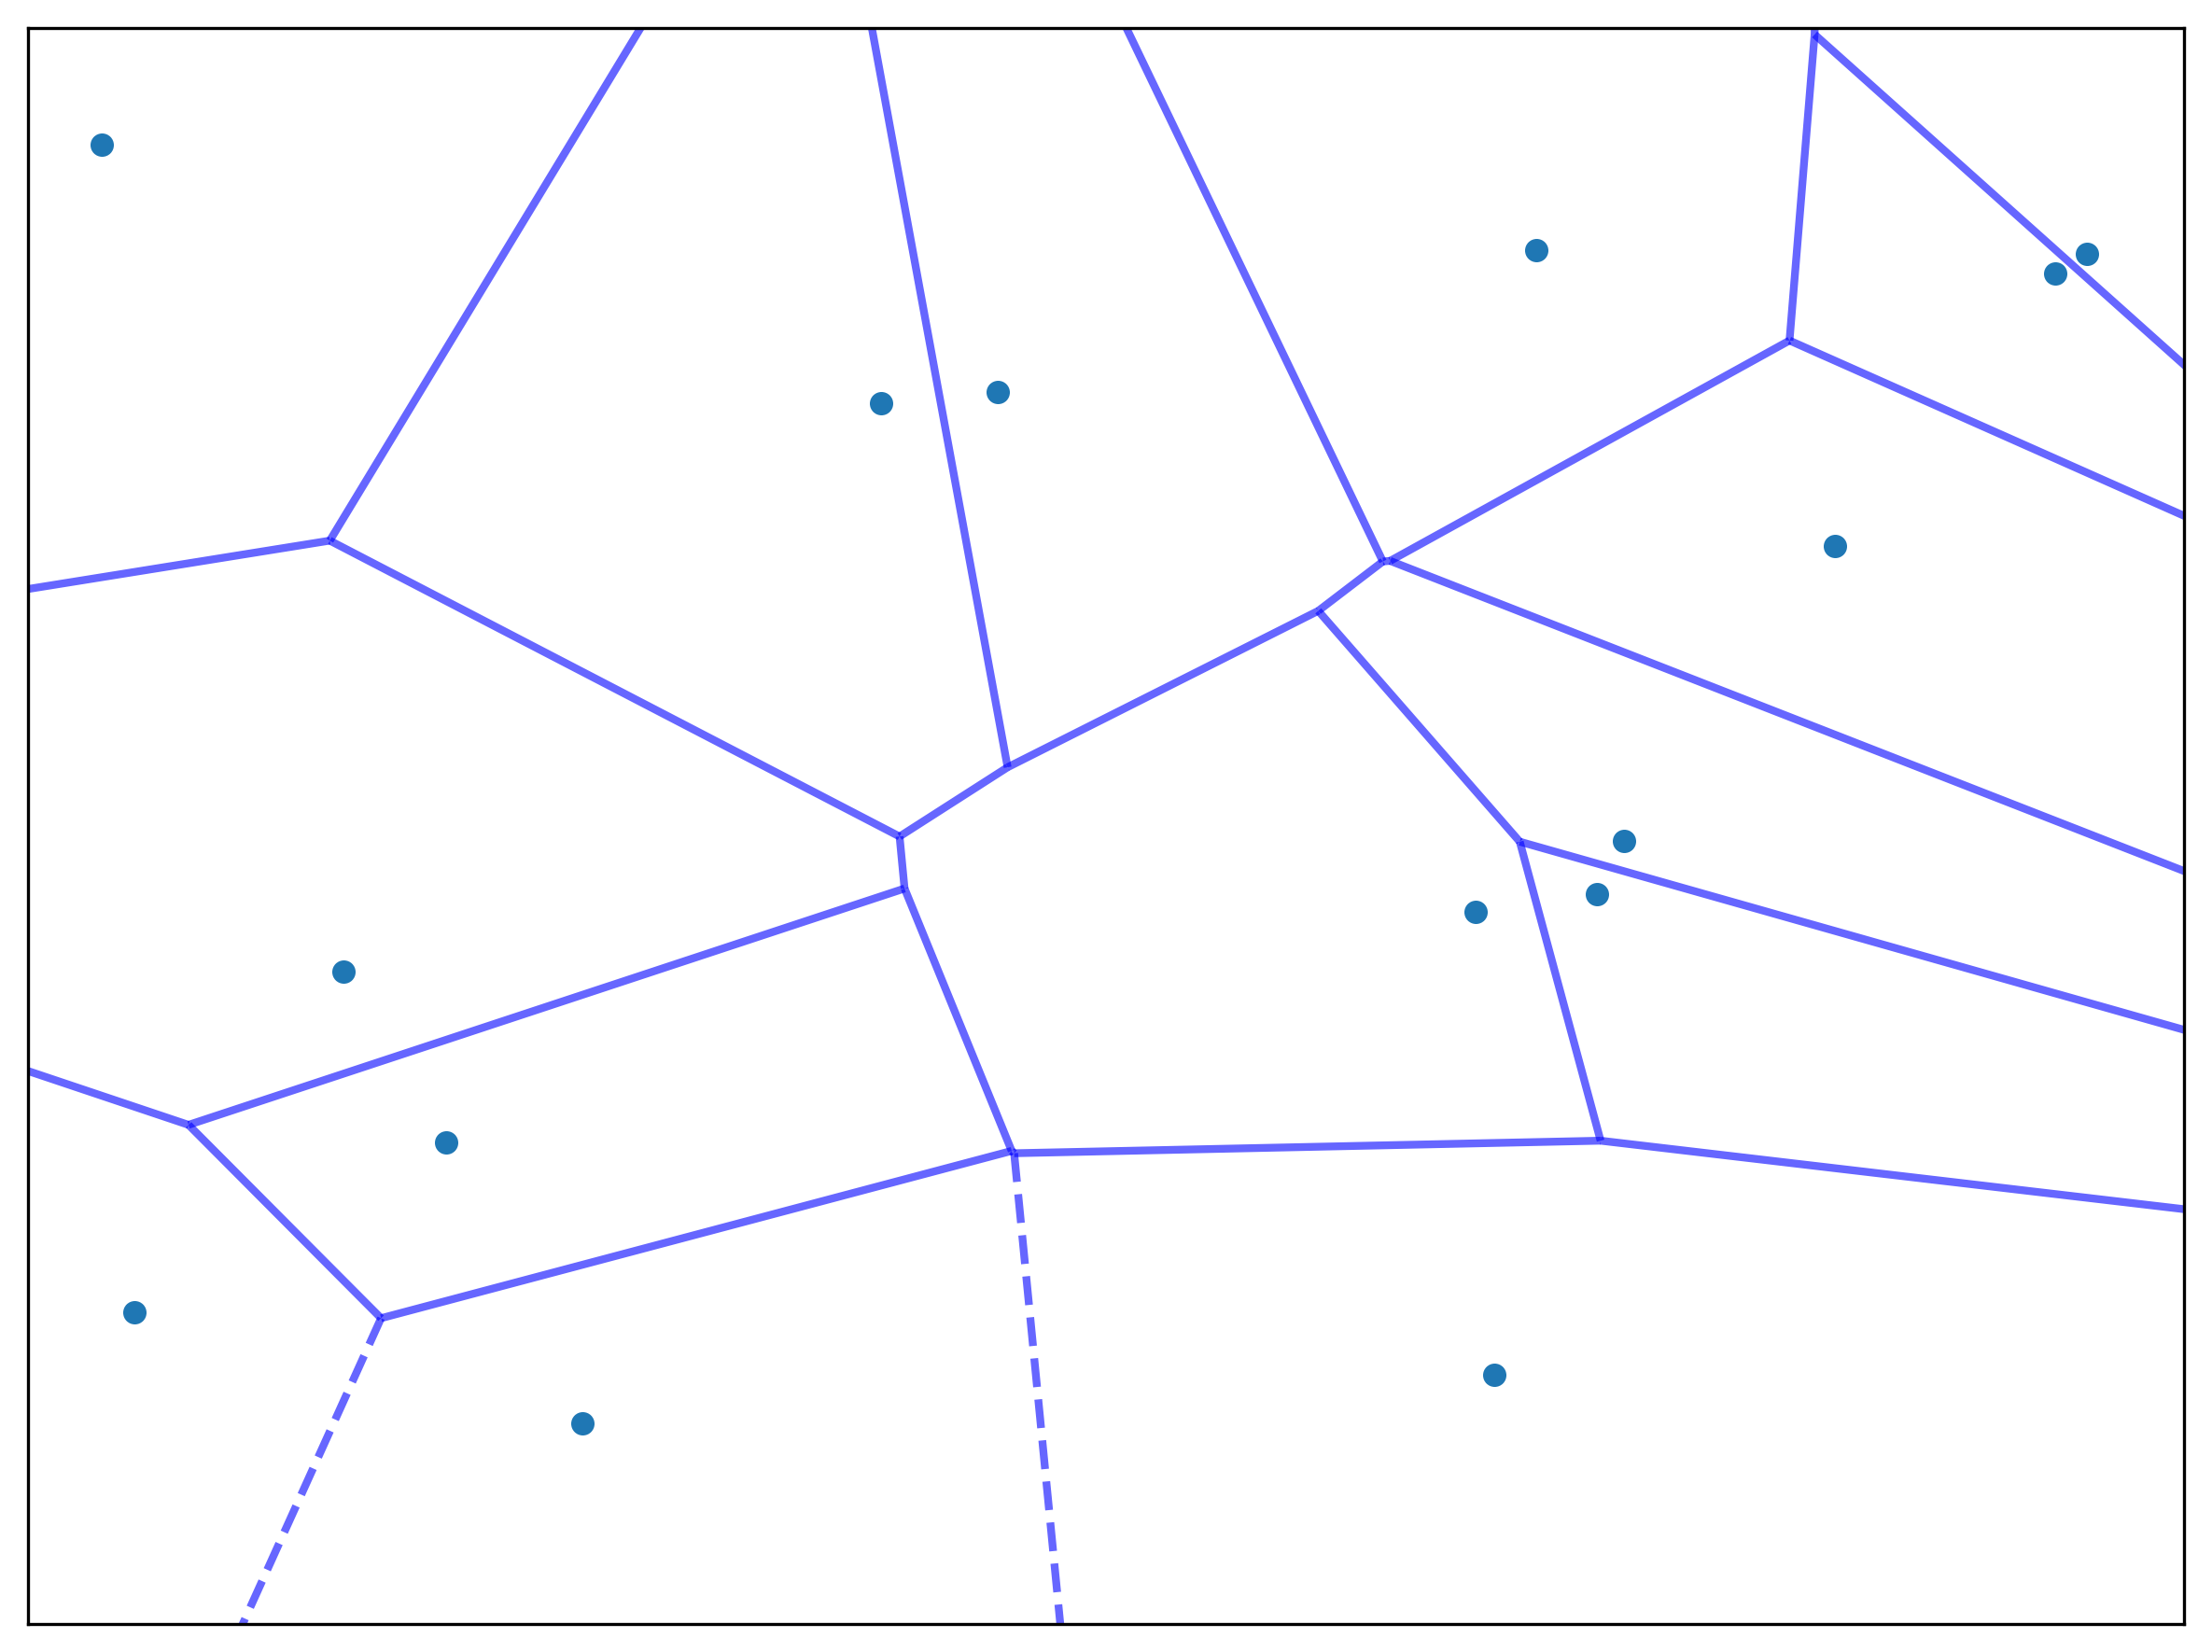
\includegraphics[width=0.4\textwidth]{img/voronoi_example.png}
    \caption{A bázisállomások lefedettségi területének becslésére használt Voronoi-tesszelláció sematikus ábrázolása. A kék pontok a bázisállomásokat, a vonalak a becsült cellahatárokat jelölik.}
    \label{fig:voronoi}
\end{figure}

\subsubsection{Tipikus adatszerkezet és mezők}

A kutatási célú CDR-adatbázisok szerkezete általában relációs modellt használ, amely lehetővé teszi a hatékony elemzést. A következő táblaszerkezet tekinthető általánosnak \cite{pinter2020artificial, pinter2022awakening}:

\begin{itemize}
    \item \textbf{Eseménytábla (CDR Raw):} A tranzakciós tábla, ahol minden sor egy hálózati eseményt ír le. Kulcsmezői: az előfizető pszeudoazonosítója (\textit{Hashed ID}), a cella azonosítója (\textit{Cell ID}), a pontos időbélyeg (\textit{Timestamp}), valamint az esemény típusa (hívás, SMS, adat).

    \item \textbf{Cella metaadatok (Cell Dimension):} A hálózati topológiát leíró tábla, amely tartalmazza a cella azonosítóját és a bázisállomás földrajzi koordinátáit (szélesség, hosszúság). A pontos lefedettségi terület becslésére gyakran Voronoi-tesszellációt alkalmaznak \cite{pinter2020artificial}.

    \item \textbf{Előfizetői attribútumok (Subscriber Dimension):} Az anonim azonosítóhoz kapcsolt statikus adatok. Adatvédelmi okokból ez gyakran korlátozott, de tartalmazhat technikai jellegű információkat, mint például az eszköz típusa (TAC kód alapján) vagy az előfizetés jellege (prepaid/postpaid) \cite{pinter2022awakening}.

    \item \textbf{Származtatott mobilitási metrikák (Derived Features):} Az elemzések során előállított aggregált tábla, amely időszakonként tartalmazza a felhasználókra számított mutatókat (pl.\ gyrációs sugár, entrópia, otthon/munkahely becsült helye) \cite{pinter2021evaluating}.
\end{itemize}

Az adatok térbeli elemzését gyakran segíti egy kiegészítő állomány, amely a cellákat közigazgatási egységekhez (pl.\ kerületek) vagy egységes rácshálóhoz rendeli \cite{rhoads2020measuring}. A 6.\ fejezetben bemutatott rendszerterv ezt az általános modellt adaptálja az YJMob100K rácsalapú szerkezetére.

\subsubsection{Adatminőség, korlátok és etikai keretek}

A nyílt vagy harmadik fél által biztosított CDR-állományok elemzésekor több technikai és módszertani korlátot kell figyelembe venni:

\begin{itemize}
    \item \textbf{Reprezentativitás:} Az adatok általában egyetlen szolgáltatótól származnak, így a piaci részesedéstől függően a teljes populáció csak részben reprezentált \cite{pinter2022awakening}.

    \item \textbf{Passzív adatok hiánya:} A kutatói adatkészletek jellemzően csak az aktív (számlázott) eseményeket tartalmazzák, a passzív cellaváltásokat (\textit{handover}) nem. Ez ritkább mintavételezést eredményez, ami megnehezíti a folyamatos mozgáskövetést \cite{pinter2022awakening}.

    \item \textbf{Térbeli felbontás:} A cellák eltérő mérete miatt a sűrűn lakott városi területek mobilitása pontosabban, míg a vidéki területeké durvábban becsülhető \cite{gonzalez2008understanding}.
\end{itemize}

Az egyéni visszakövetés elkerülése érdekében pszeudo-azonosítókat használnak, és a kutatók számára gyakran csak minimális demográfiai adatokat tesznek hozzáférhetővé, ahogy azt a Data4Refugees projekt esetében is láthatjuk \cite{zhang2019connected}.
